\documentclass[12pt]{article}
\usepackage[russian]{babel}
\usepackage{geometry}

%библиотеки для задания 2
\usepackage{graphicx}
\usepackage{caption}

\usepackage{enumitem}

%нестандартные математические обозначения
\usepackage{amssymb}
\usepackage{amsmath}

%различные цветовые модели
\usepackage[usenames]{color}
\usepackage[dvipsnames,table]{xcolor}
\usepackage{colortbl}

\usepackage{listings}
\usepackage{listingsutf8}
\usepackage[T2A]{fontenc}
\newcommand{\listingsttfamily}{\usefont{T2A}{PTMono-TLF}{m}{n}}

\lstset{
	language=C,                % choose the language of the code
	numbers=left,                   % where to put the line-numbers
	stepnumber=1,                   % the step between two line-numbers.        
	numbersep=5pt,                  % how far the line-numbers are from the code
	backgroundcolor=\color{black},  % choose the background color. You must add \usepackage{color}
	commentstyle=\color{Gray},
	basicstyle=\listingsttfamily\color{Gray},
	keywordstyle=\color{BurntOrange},
	stringstyle=\color{YellowGreen},
	showspaces=false,               % show spaces adding particular underscores
	showstringspaces=false,         % underline spaces within strings
	showtabs=false,                 % show tabs within strings adding particular underscores
	tabsize=4,                      % sets default tabsize to 2 spaces
	captionpos=b,                   % sets the caption-position to bottom
	breaklines=true,                % sets automatic line breaking
	breakatwhitespace=true,         % sets if automatic breaks should only happen at whitespace
	title=\lstname, 
	inputencoding=utf8,                % show the filename of files included with \lstinputlisting;
	extendedchars=\true,
	keepspaces=true
}

%параметры документа
\geometry{top=2cm, bottom=2cm, left=1cm, right=1cm}
\textheight=24cm
\textwidth=18cm
\flushbottom 

\oddsidemargin=0pt 
\topmargin=-1.5cm 
\parskip=0pt
\parindent=24pt 

\tolerance=2000 

\begin{document}
	\begin{center}
		{\parskip=1cm
			МИНИСТЕРСТВО НАУКИ И ВЫСШЕГО ОБРАЗОВАНИЯ РОССИЙСКОЙ ФЕДЕРАЦИИ
			
			ФЕДЕРАЛЬНОЕ ГОСУДАРСТВЕННОЕ БЮДЖЕТНОЕ ОБРАЗОВАТЕЛЬНОЕ УЧРЕЖДЕНИЕ ВЫСШЕГО ОБРАЗОВАНИЯ
			
			{\bf«БЕЛГОРОДСКИЙ ГОСУДАРСТВЕННЫЙ ТЕХНОЛОГИЧЕСКИЙ УНИВЕРСИТЕТ им. В. Г. Шухова»\\(БГТУ им. В. Г. Шухова)}
			
			
			\begin{figure}[bh]
			\noindent\centering{
				
\includegraphics[width=100mm]{images/start_logo.png}
				\captionsetup{labelformat=empty}
			}
			\end{figure}
			Кафедра программного обеспечения вычислительной техники и автоматизированных систем
		}
		{\parskip=0.25cm
			{\Large 
				{\bf Лабораторная работа №6}
			
				по дисциплине: <<Алгоритмы и структуры данных>>
			
				по теме: {\bf <<Структуры данных <<стек>> и <<очередь>> (С)>>}
			}
		}
	\end{center}
	\begin{flushright}
		{\parskip=3cm Выполнил/a: ст. группы ПВ-231}
		
		Чупахина София Александровна
		
		Проверил:
		
		Акиньшин Даниил Иванович
	\end{flushright}
	\begin{center}
		{\parskip=3cm Белгород, 2024}
	\end{center}
	\newpage
	
	{\bf Цель работы:} изучить СД типа <<стек>> и <<очередь>>, научиться их программно реализовывать и использовать.
	
	
	{\bf Задания:}
	
	\setlist[3]{noitemsep} % sets the itemsep and parsep for all level two lists to 0
	
	\begin{enumerate}
	
	\item Для СД типа  <<стек>> и <<очередь>> определить:
	
		\begin{enumerate}
	
			\item Абстрактный уровень представления СД:
			
			\begin{enumerate}
	
				\item Характер организованности и изменчивости, 
	
				\item Набор допустимых операций.
			
			\end{enumerate}
	
	
			\item Физический уровень представления СД:
			
			\begin{enumerate}
	
				\item Схему хранения;
	
				\item Объем памяти, занимаемый экземпляром СД;
	
				\item Формат внутреннего представления СД и способ его  интерпретации;
				
				\item Характеристику допустимых значений;
				
				\item Тип доступа к элементам.
				
			\end{enumerate}
			
			\item Логический уровень представления СД. Способ описания СД и экземпляра СД на языке программирования.
	
		\end{enumerate}
	
	\item Реализовать СД типа <<стек>> и <<очередь>> в соответствии с вариантом индивидуального задания в виде модуля;
	
	\item Разработать  программу,  моделирующую  вычислительную  систему с постоянным шагом по времени (дискретное время) в соответствии с вариантом индивидуального задания (табл.16) с использованием модуля, полученного в результате выполнения пункта 2. Результат работы программы представить в виде таблицы 15. В первом столбце указывается время моделирования $0, 1, 2, …, N$. Во втором — для каждого момента времени указываются имена объектов (очереди — $F_1, F_2, …, F_N$; стеки — $S_1, S_2, …, S_M$; процессоры — $P_1, P_2, …, P_K$), а в третьем — задачи (имя, время), находящиеся в объектах.
	
	\end{enumerate}
	
	\setcounter{secnumdepth}{-1} 
	\tableofcontents
	\newpage
	
	{\parskip=0.15cm
	
	\section{Задание 1:}
	\label{task_1}
	Опишем СД типа <<стек>> и <<очередь>>.
	
	\subsection{Абстрактный уровень:}
	\label{task_1_1}
	\subsubsection{Задание 1.1.1:}
	\label{task_1_1_1}
	
	Как CД типа <<стек>>, так и СД типа <<очередь>> являются линейными СД. Как и рассматриваемые ранее СД типа <<массив>> и <<линейный список>>, они отображают некую упорядоченную последовательность элементов, и для каждого из них, кроме первого и последнего, существует предыдущий и следующий. СД типа <<стек>> и <<очередь>> могут быть реализованы для любого типа элементов. Специфика СД типа <<стек>> и <<очередь>> в том, что для них невозможна перезапись и чтение элемента по произвольному индексу (как для массива), а также включение и исключение элемента на произвольную позицию (как для линейных списков). В СД типа стек включать, исключать и считывать элемент можно только с одной определенной позиции, которая называется вершиной стека. Таким образом, последний включенный элемент будет ближе всего к вершине стека, из которой проводится исключение, и потому при исключении он будет извлечен первым. Это свойство дало стеку сокращенное название LIFO (от англ. Last In, First Out). В СД типа очередь элементы всегда включаются с одной позиции, которая называется хвостом очереди, и исключаются и считываются с другой позиции, которая называется головой очереди. Только что включенный с хвоста элемент отделяется от головы всеми теми элементами, которые были включены в список до него. По аналогии со стеком, очередь имеет указывающее на это свойство сокращенное название FIFO (от англ. First In, First Out).
	
	Обычно роль вершины, головы или хвоста отдается первому или последнему элементу массива.
	
	<<Стек>> и <<очередь>> являются динамическими СД: несмотря на невозможность перезаписи и осуществление включения и исключения только с одной позиции (эти позиции совпадают для стека и не совпадают для очереди) в нем могут меняться как сами элементы, так и их количество. Количество элементов ограничено только способом реализации структуры; этот аспект подробнее рассмотрим в задании 1.2. 
	
	\subsubsection{Задание 1.1.2:}
	\label{task_1_1_2}
	СД типа <<стек>> и <<очередь>> не реализованы в языках программирования по умолчанию, то есть являются производными структурами данных. Тем не менее, для каждой из них существуют операции, которые должны быть реализованы по определению. Для СД типа <<стек>> это операции:
	
	\begin{enumerate}
	\item Инициализация.
	\item Включение элемента.
	\item Исключение элемента.
	\item Чтение элемента.
	\item Проверка пустоты стека.
	\item Уничтожение стека.
	\end{enumerate}
	
	А для СД типа <<очередь>> --- следующие операции:
	\begin{enumerate}
	\item Инициализация.
	\item Включение элемента.
	\item Исключение элемента.
	\item Чтение элемента (с головы очереди).
	\item Проверка пустоты очереди.
	\item Уничтожение очереди.
	\end{enumerate}
	
	\subsection{Физический уровень:}
	\label{task_1_2}
	\subsubsection{Задание 1.2.1:}
	\label{task_1_2_1}
	Для СД типа <<стек>> и <<очередь>> может использоваться как прямоугольная, так и связная схема хранения. При использовании прямоугольной схемы для хранения элементов стека или очереди используется массив; тогда последовательности битов, представляющие нулевой, первый, второй и так далее элемент, идут друг за другом по возрастанию индекса подряд, без разделителей. Точно так же для реализации стека или очереди может использоваться связная схема хранения --- тогда элементы этих СД будут храниться в связном списке. В таком случае значение каждого элемента включено в структуру типа <<запись>>, которая хранит также указатель на следующий элемент (для односвязного списка) или указатели на следующий и на предыдущий элемент (для двусвязного списка). В любом случае, над СД типа <<стек>> и <<очередь>> реализуются также и функции, ограничивающие доступ к элементами массива или списка по умолчанию и обеспечивающие выполнение ключевых условий: включение, исключение или чтение элемента только с вершины стека; включение элемента только с хвоста и исключение и чтение только с головы для очереди.
	
	\subsubsection{Задание 1.2.2:}
	\label{task_1_2_2}
	Количество памяти, занимаемой СД типа <<стек>> или <<очередь>>, зависит от того, какое количество памяти занимает его базовый тип, есть ли необходимость хранить дополнительную информацию (указатели на другие элементы для связной схемы хранения) о каждом элементе, и сколько элементов содержит СД. Если базовый тип занимает $T$ байт, для каждого элемента необходимо также хранить $P$ ($P$ также может быть равно 0) указателей типа {\it unsigned long}, занимающего 8 байт, а список содержит $K$ элементов, то количество памяти, занимаемой экземпляром любой из этих СД, будет равно $(T+P)*K$ байт.
	
	\subsubsection{Задание 1.2.3:}
	\label{task_1_2_3}
	Если СД типа <<стек>> или <<очередь>> с длиной K использует последовательную схему хранения, то значение этой структуры хранится как $K$ идущих подряд последовательностей битов, кодирующих значения элементов СД в соответствии с правилами для данного базового типа. Для связных же вариантов реализации каждый узел (структура с одним полем <<значение элемента>> и несколькими полями <<указатели>>) хранится независимо друг от друга, и значения в полях узла также могут храниться в памяти компьютера не подряд (либо в порядке, отличном от заданного). Значение элемента переводится в двоичный код в зависимости от базового типа; указатели кодируются как положительные целые числа --- переводятся в двоичную систему счисления и дополняются нулями слева до размера в 8 байт.

	\subsubsection{Задание 1.2.4:}
	\label{task_1_2_4}
	Диапазоны допустимых значений СД типа <<стек>> и <<очередь>> связаны с диапазонами допустимых значений их базовых элементов. Если рассматривать стек или очередь некоторой фиксированной длины $K$, то количество возможных значений для экземпляров этих СД равно возведенному в степень $K$ количеству возможных значений для их базового элемента. Соответственно, для СД типа <<стек>> или <<очередь>> количество возможных значений равно сумме количеств возможных значений этих СД с длинами от 0 до max, где max --- максимальная длина стека или очереди (однозначно определенная в случаях, когда эти СД реализованы на массиве). Обозначая количество допустимых значений как CAR (кардинальное число), получим формулу $CAR(STACK) = CAR(FIFO) = CAR(BaseType)^0 + CAR(BaseType)^1 +… + CAR(BaseType)^max$.
	
	\subsubsection{Задание 1.2.5:}
	\label{task_1_2_5}
	СД типа <<стек>> и <<очередь>> имеют ограниченный доступ к элементам. Для стека чтение осуществляется только с его вершины, для очереди --- только с ее головы. Соответственно, чтобы получить некоторый (не вершинный) элемент стека, нужно исключить из него все элементы, которые отделяют его от вершины, а чтобы получить некоторый (не головной) элемент очереди, нужно исключить из нее все элементы, которые отделяют его от головы. С этой точки зрения логичнее будет сказать, что доступ к элементам в этих СД последователен.
	
	\subsection{Логический уровень:}
	\label{task_1_3}
	СД типа <<стек>> и <<очередь>> не являются встроенными, и потому сначала необходимо реализовать их, выбрав один из способов отображения. Только после этого их можно описать на логическом уровне (представить на языке программирования). Приведем здесь описания для той реализации, которая будет выполнена в задании 2 этой лабораторной работы. Стек отображается на последовательный линейный список, и его вершиной является первый элемент этого списка; кольцевая очередь отображается на массив в динамической памяти. Пока что мы не реализовали функции для работы с этими СД, и заполнение стека и очереди значениями, ка ки задание основных параметров, будет происходить более примитивными способами.
	
	\lstinputlisting{../АСД 6 си/stack/example.c} 
		
	\lstinputlisting{../АСД 6 си/fifo/example.c} 
	
	\begin{center}
	{\bf Индивидуальное задание; вариант 21}
	\end{center}
	{\bf Модуль 10 (для стека):} Стек на ПЛС. Вершина стека – первый элемент ПЛС.
	
	{\bf Реализация на языке C:}
	
	{\it \#if !defined(\_\_STACK10\_H)
		
		\#define \_\_STACK10\_H
		
		\#include "list6.h" // Смотреть лаб. раб. №5
		
		const StackOk = ListOk;
		
		const StackUnder = ListUnder;
		
		const StackOver = ListNotMem;
		
		int   StackError; // Переменная ошибок
		
		typedef List Stack;
		
		void InitStack(Stack *s, unsigned Size);  /* Инициализация стека */
		
		void PutStack(Stack *s, void *E); // Поместить элемент в стек      
		
		void GetStack(Stack *s, void *E); // Извлечь элемент из стека  
		
		int EmptyStack(Stack s);  // Проверка: стек пуст?
		
		void ReadStack(Stack s, void *E);  /* Прочитать элемент из вершины стека */
		
		void DoneStack(Stack *s); // Уничтожить стек
		
		\#endif}
	
	{\bf Модуль 11 (для очереди):} Очередь (кольцевая) на массиве в динамической памяти.
	
	{\it \#if !defined(\_\_FIFO11\_H)
		
	\#define \_\_FIFO11\_H
	
	const FifoOk = 0;
	
	const FifoUnder = 1;
	
	const FifoOver = 2;
	
	int FifoError; // Переменная ошибок
	
	typedef void *BaseType; 
	
	typedef struct Fifo
	
	\{
	
		BaseType *Buf;
	
		unsigned SizeBuf; // Максимальная длина очереди
	
		unsigned SizeEl; // Размер элемента очереди
	
		unsigned Uk1; // Указатель на «голову» очереди
	
		unsigned Uk2; // Указатель на «хвост» очереди
	
		unsigned N;   // Количество элементов очереди
	
	\};
	
	void InitFifo(Fifo* f, unsigned SizeEl, unsigned SizeBuf);    
	
	// Инициализация очереди
	
	void PutFifo(Fifo *f, void *E); /* Поместить элемент в очередь */
	
	void GetFifo(Fifo *f, void *E); // Извлечь элемент из очереди 
	
	void ReadFifo(Fifo *f, void *E);  // Прочитать элемент                  
	
	int  EmptyFifo(Fifo *f); // Проверка, пуста ли очередь?
	
	void DoneFifo(Fifo *f); // Разрушить очередь
	
	\#endif}
	
	{\bf Задача 2:} Система состоит из процессора $P$, трех очередей $F_0,  F_1,  F_2$ и стека $S$. В систему поступают запросы. Запрос можно представить записью.
	
	typedef struct TInquiry
	
	{\it \{  
		
		char Name[10]; // имя запроса
		
		unsigned Time; // время обслуживания
		
		char P; /* приоритет задачи: 0 — высший, 1 — средний, 2 — низший */
		
	\}};	
	
	Поступающие запросы ставятся в соответствующие приоритетам очереди. Сначала обрабатываются задачи из очереди $F_0$. Если она пуста, можно обрабатывать задачи из очереди $F_1$. Если и она пуста, то можно обрабатывать задачи из очереди $F_2$. Если все очереди пусты, то система находится в ожидании поступающих задач (процессор свободен), либо в режиме обработки предыдущей задачи (процессор занят). Если обрабатывается задача с низшим приоритетом и поступает задача с более высоким приоритетом, то обрабатываемая помещается в стек и может обрабатываться тогда и только тогда, когда все задачи с более высоким приоритетом уже обработаны.
	
	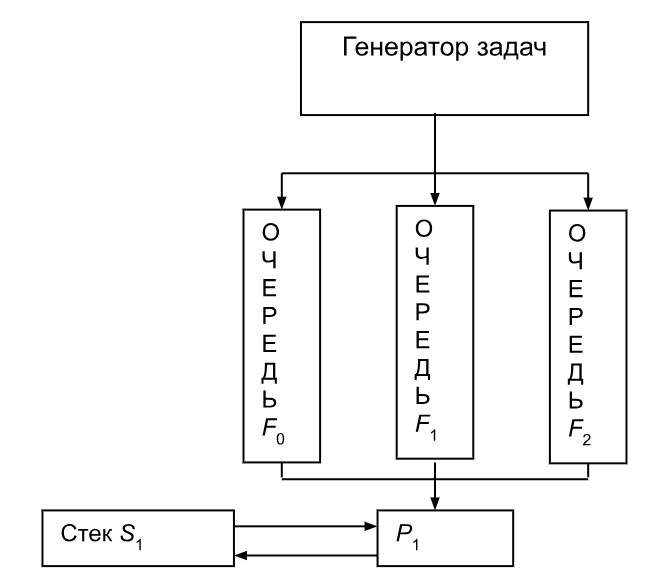
\includegraphics[width=120mm]{images/sheme.png}
	
	\section{Задание 2:}
	\label{task_2}
	
	Начнем с реализации модуля для работы со стеком. Стек должен быть реализован на последовательном линейном списке, однако в прошлой лабораторной работе мы реализовали модуль для работы с односвязными линейными спиками. Значит, перед тем, как приступать к работе со стеками, необходимо написать модуль для ПЛС. 
	
	Как обычно, разделим код на два файла: заголовочный и  реализации. В заголовочном файле зададим константы с кодами трех основных ошибок, которые могут возникнуть в ходе работы со списками: ListNotMem --- для выделения места под новый элемент нет места в списке свободных элементов в массиве MemList; ListUnder --- попытка получить доступ к элементу, в то время как пуст либо список, либо текущий указатель; ListEnd --- в ходе перебора элементов списка был достигнут его конец. Под хранение кода ошибки отводится переменная. После этого дадим название используемым типам данных: ptrel --- беззнаковое целое число, номер элемента списка, к которому идет обращение на данный момент; List --- структура, хранящая массив с элементами типа void* (его размер задан константой), номер текущего элемента, их общее количество и размер базового типа. Только после этого будут объявлены прототипы функций для работы со списками. 
	
	\lstinputlisting{../АСД 6 си/SLList/SLList.h} 
	
	Реализация функций будет вынесена в отдельный файл со следующим содержанием.
	
	{\bf Примечание:} функция PutList подразумевает, что элемент вставляется после элемента, номер которого хранит рабочий указатель, поэтому, чтобы вставить элемент в самое начало списка, рабочий указатель должен быть равен нулю, при условии, что нулю не равен стартовый указатель. Функция GetList подразумевает, что удаляется тот элемент, номер которого хранит рабочий указатель, поэтому попытка удаления элемента, когда указатель равен 0, приведет к выходу с кодом ошибки ListEnd. Нумерация начинается с единицы, при этом в массиве элементы хранятся, начиная с нулевого элемента: данное смещение учитывается в коде функций.
	
	\lstinputlisting{../АСД 6 си/SLList/SLList.c} 

	Теперь можем перейти к стеку. Также разобьем этот модуль на два файла. В предложенной реализации, структура <<стек>> ---  переименование структуры <<список>>, и множество ошибок для нее --- подмножество множества ошибок для структуры <<список>> (но эти множества не одинаковы; в отличие от списка, для стека не имеет смысл ошибка <<достигнут конец>>). Функции для стека тоже в каком-то смысле подмножеством функций списка.
	
	\lstinputlisting{../АСД 6 си/stack/stack.h} 
	
	Также и реализация этих функций сводится к вызову аналогичных функций для списка, на который отображен стек, с единственной модификацией --- указатель после выполнения каждой из них должен иметь значение 1 (указывать на первый элемент последовательности), поскольку вершиной стека считается первый элемент списка. При инициализации стека указатель приравнивается к 1: далее мы считаем, что он равен 1 по умолчанию, и устанавливаем его в 1 после вызова функций, которые могут его изменить. Единственный случай, когда мы устанавливаем его в 0 --- включение элемента в стек (то есть вставка не после, а перед текущим первым элементом списка, которая требует именно такого значения указателя). А так как при работе со списками после включения элемента значение указателя возрастает на 1, нет нужды перезаписывать его как 1 повторно.
	
	\lstinputlisting{../АСД 6 си/stack/stack.c} 
	
	Для нормальных (не вызывающих ошибки и аварийного завершения) сценариев большинства функций (за исключением уничтожающей стек функции DoneStack), можно составить автоматизированные тесты и вынести их в отдельный файл тестирования. Будем тестировать функции по порядку; после того, как они протестированы, их можно использовать в тестах дальнейших функций. Запустив программу, можем самостоятельно убедиться, что все тесты прошли успешно:
	
	\lstinputlisting{../АСД 6 си/stack/stack_test.c} 
	
	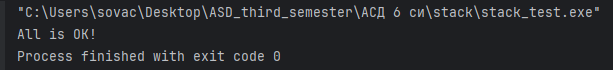
\includegraphics[width=150mm]{images/stack_test.png}
	
	Перейдем к очереди. Кольцевая очередь реализуется непосредственно на массиве. Также определяется список ошибок: FifoUnder, если происходит попытка извлечь/прочесть элемент из пустой очереди, и FifoOver, если количество элементов в очереди превышает количество элементов, для которого изначально была отведена память. После этого задается структура <<очередь>> с шестью полями: указатель на начало массива, элементы которого --- пустые указатели на реальные элементы очереди; максимальное количество элементов, для хранения которых выделяется память при инициализации, размер базового типа в байтах, индекс элемента в массиве, являющегося головой очереди, индекс элемента в массиве, являющегося хвостом очереди, переменная, хранящая количество элементов в массиве.
	
	\lstinputlisting{../АСД 6 си/fifo/fifo.h} 
	
	Работая со стеком на последовательном линейном списке, мы условились, что его врешиной будет первый элемент списка, и, включая или исключая элемент, сдвигали уже имеющиеся относительно начала. В данной реализации очереди мы поступим противоположным образом: элементы будут оставаться на прежних позициях, но указатели на голову и хвост будут смещаться таким образом, что указатель на голову всегда указывает на последний (головной) элемент очереди, указатель на хвост --- на позицию, следующую за первым (хвостовым) элементом. При операции включения указатель на хвост увеличивается на 1, при операции исключения увеличивается на 1 указатель на голову. Таким образом, област ьмежду указателями, в которой и будут храниться элементы, будет постепенно смещаться от его левого края к правому, оставляя <<по бокам>> неиспользованное место. Но очередь, которую мы реализуем, является кольцевой; достигая конца массива, указатель переходит на его начало. Таким образом, очередь может использовать область массива <<по бокам>>, а последовательность элементов может быть распределена так, что часть ее продолжается от головы до правого конца массива, а вторая часть --- от начала массива до хвоста. Это учитывается в теле функций включения и исключения.
	
	\lstinputlisting{../АСД 6 си/fifo/fifo.c}
	
	Аналогичным образом проведем тестирование для очереди (нормальных сценариев всех функций, кроме DoneFifo). Эти тесты также прошли успешно: 
		
	\lstinputlisting{../АСД 6 си/fifo/fifo_test.c} 

	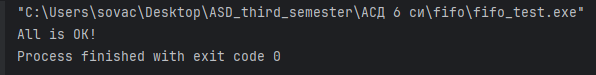
\includegraphics[width=150mm]{images/fifo_test.png}
	
	\section{Задание 3:}
	\label{task_3}
	
	Теперь, когда модули для СД типа <<стек>> и <<очередь>>, реализованы, можем перейти к решению задачи: моделированию вычислительной системы, описанной выше. Сначала объявим структуры для отображения объектов, использующихся в модели системы,  помимо стека и очередей --- процессора и генератора задач. Затем объявим функции, отвечающие за некоторые ключевые шаги (к каждой из них написан комментарий, объясняющий, за какое действие в системе она отвечает), и функции для вывода задач, содержащихся в той или иной структуре. Все эти функции будут объединены в функции makeTact, которая будет выполнять вышеописанные шаги в зависимости от текущего наполнения очередей, стека, процессора, и выводить их на экран в конце такта. В теле функции main все составляющие модели инициализируются, и функция makeTact запускается в цикле заданное количество раз.
	
	\lstinputlisting{../АСД 6 си/task/task_updated.c} 
	
	Пример, показывающий, как организован вывод, можно увидеть на скриншотах ниже. На них запечатлен вывод после выполнения десяти тактов: 
	
	\parbox[с][130mm][c]{50mm}{
		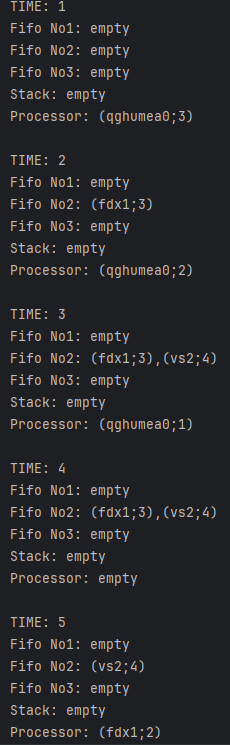
\includegraphics[height=130mm]{images/task1.png}
	}
	\hspace{1cm}
	\parbox[с][130mm][c]{60mm}{
		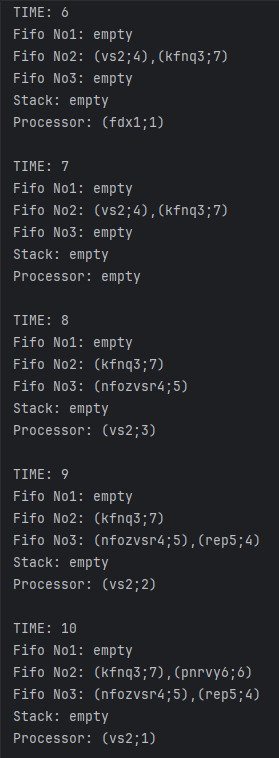
\includegraphics[height=130mm]{images/task2.png}
	}
	
	Перенесем в таблицу выведенные данные.
	
	\begin{tabular}{|c|c|l|}
		\hline
		{\bf Время} & {\bf Объекты} & {\bf Задачи}\\
		\hline
		1 & F1 & empty \\
		\cline{2-3}
		& F2 & empty \\
		\cline{2-3}
		& F3 & empty \\
		\cline{2-3}
		& S & empty \\
		\cline{2-3}
		& P & (qghumea0;3) \\
		\hline
		
		2 & F1 & empty \\
		\cline{2-3}
		& F2 & (fdx1;3) \\
		\cline{2-3}
		& F3 & empty \\
		\cline{2-3}
		& S & empty \\
		\cline{2-3}
		& P & (qghumea0;2) \\
		\hline
		
		
		3 & F1 & empty\\ 
		\cline{2-3}
		& F2 & (fdx1;3),(vs2;4)\\
		\cline{2-3}
		& F3 & empty\\
		\cline{2-3}
		& S & empty\\
		\cline{2-3}
		& P & (qghumea0;1)\\
		\hline
		
		
		4 & F1 & empty\\ 
		\cline{2-3}
		& F2 & (fdx1;3),(vs2;4)\\
		\cline{2-3}
		& F3 & empty\\
		\cline{2-3}
		& S & empty\\
		\cline{2-3}
		& P & empty\\
		\hline
		
		
		5 & F1 & empty\\ 
		\cline{2-3}
		& F2 & (vs2;4)\\
		\cline{2-3}
		& F3 & empty\\
		\cline{2-3}
		& S & empty\\
		\cline{2-3}
		& P & (fdx1;2)\\
		\hline
		
		6 & F1 & empty\\ 
		\cline{2-3}
		& F2 & (vs2;4),(kfnq3;7)\\
		\cline{2-3}
		& F3 & empty\\
		\cline{2-3}
		& S & empty\\
		\cline{2-3}
		& P & (fdx1;1)\\
		\hline
		
		7 & F1 & empty\\ 
		\cline{2-3}
		& F2 & (vs2;4),(kfnq3;7)\\
		\cline{2-3}
		& F3 & empty\\
		\cline{2-3}
		& S & empty\\
		\cline{2-3}
		& P & empty\\
		\hline
		
		8 & F1 & empty\\ 
		\cline{2-3}
		& F2 & (kfnq3;7)\\
		\cline{2-3}
		& F3 & (nfozvsr4;5)\\
		\cline{2-3}
		& S & empty\\
		\cline{2-3}
		& P & (vs2;3)\\
		\hline
	\end{tabular}
	
	\begin{tabular}{|c|c|l|}
		\hline
		9 & F1 & empty\\ 
		\cline{2-3}
		& F2 & (kfnq3;7)\\
		\cline{2-3}
		& F3 & (nfozvsr4;5),(rep5;4)\\
		\cline{2-3}
		& S & empty\\
		\cline{2-3}
		& P & (vs2;2)\\
		\hline
	
		10 & F1 & empty\\ 
		\cline{2-3}
		& F2 & (kfnq3;7),(pnrvy6;6)\\
		\cline{2-3}
		& F3 & (nfozvsr4;5),(rep5;4)\\
		\cline{2-3}
		& S & empty\\
		\cline{2-3}
		& P & (vs2;1)\\
		\hline
		
		11 & F1 & empty\\ 
		\cline{2-3}
		& F2 & (kfnq3;7),(pnrvy6;6)\\
		\cline{2-3}
		& F3 & (nfozvsr4;5),(rep5;4)\\
		\cline{2-3}
		& S & empty\\
		\cline{2-3}
		& P & empty\\
		\hline
		
		12 & F1 & empty\\ 
		\cline{2-3}
		& F2 & (pnrvy6;6)\\
		\cline{2-3}
		& F3 & (nfozvsr4;5),(rep5;4),(ys7;4)\\
		\cline{2-3}
		& S & empty\\
		\cline{2-3}
		& P & (kfnq3;6)\\
		\hline
		
		13 & F1 & empty\\ 
		\cline{2-3}
		& F2 & (pnrvy6;6)\\
		\cline{2-3}
		& F3 & (nfozvsr4;5),(rep5;4),(ys7;4)\\
		\cline{2-3}
		& S & (kfnq3;6)\\
		\cline{2-3}
		& P & (pevi8;3)\\
		\hline
		
		14 & F1 & empty\\ 
		\cline{2-3}
		& F2 & (pnrvy6;6),(mznim9;2)\\
		\cline{2-3}
		& F3 & (nfozvsr4;5),(rep5;4),(ys7;4)\\
		\cline{2-3}
		& S & (kfnq3;6)\\
		\cline{2-3}
		& P & (pevi8;2)\\
		\hline
		
		15 & F1 & empty\\ 
		\cline{2-3}
		& F2 & (pnrvy6;6),(mznim9;2)\\
		\cline{2-3}
		& F3 & (nfozvsr4;5),(rep5;4),(ys7;4)\\
		\cline{2-3}
		& S & (kfnq3;6)\\
		\cline{2-3}
		& P & (pevi8;1)\\
		\hline
		
		16 & F1 & empty\\ 
		\cline{2-3}
		& F2 & (pnrvy6;6),(mznim9;2)\\
		\cline{2-3}
		& F3 & (nfozvsr4;5),(rep5;4),(ys7;4)\\
		\cline{2-3}
		& S & (kfnq3;6)\\
		\cline{2-3}
		& P & empty\\
		\hline
		
		17 & F1 & empty\\ 
		\cline{2-3}
		& F2 & (pnrvy6;6),(mznim9;2)\\
		\cline{2-3}
		& F3 & (nfozvsr4;5),(rep5;4),(ys7;4),(srenzk10;4)\\
		\cline{2-3}
		& S & empty\\
		\cline{2-3}
		& P & (kfnq3;5)\\
		\hline
	\end{tabular}
	
	\begin{tabular}{|c|c|l|}
		\hline		
		18 & F1 & empty\\ 
		\cline{2-3}
		& F2 & (pnrvy6;6),(mznim9;2)\\
		\cline{2-3}
		& F3 & (nfozvsr4;5),(rep5;4),(ys7;4),(srenzk10;4),(xtlsgyp11;4)\\
		\cline{2-3}
		& S & empty\\
		\cline{2-3}
		& P & (kfnq3;4)\\
		\hline
	
		19 & F1 & empty\\ 
		\cline{2-3}
		& F2 & (pnrvy6;6),(mznim9;2)\\
		\cline{2-3}
		& F3 & (nfozvsr4;5),(rep5;4),(ys7;4),(srenzk10;4),(xtlsgyp11;4)\\
		\cline{2-3}
		& S & empty\\
		\cline{2-3}
		& P & (kfnq3;3)\\
		\hline
		
		20 & F1 & empty\\ 
		\cline{2-3}
		& F2 & (pnrvy6;6),(mznim9;2)\\
		\cline{2-3}
		& F3 & (nfozvsr4;5),(rep5;4),(ys7;4),(srenzk10;4),(xtlsgyp11;4),(ooefxzb12;2)\\
		\cline{2-3}
		& S & empty\\
		\cline{2-3}
		& P & (kfnq3;2)\\
		\hline
	\end{tabular}
	
	\section{Вывод:}
	
	В ходе лабораторной работы дали характеристику СД типа <<стек>> и <<очередь>>, форматам их представления, реализовали по одному из них для каждой СД из них (стек на базе последовательного линейного списка с вершиной в первом элементе и кольцевую очередь на базе динамического массива), написали ряд базовых функций для работы со стеками и очередями в этом формате, а также создали модель вычислительной системы, используя, в том числе, СД типа <<стек>> и <<очередь>>.
}
\end{document}